\documentclass[results.tex]{subfiles}
\begin{document}

\newpage

\subsection{4-Regular Graph}

For the 4-Regular (Quartic) graph, the Graph Generator used the following parameters:

\begin{itemize}
\item Type of graph: 4-Regular
\item Number of vertices: 20
\item Number of edges: 40
\item Random generator seed: 1615826375197
\end{itemize}
and the model took the following parameters:
\begin{itemize}
\item Total defence quota each turn: 1.0
\item Probability with which the infection propagates: 1.0
\end{itemize}

\begin{figure}[!ht]
	\centering
	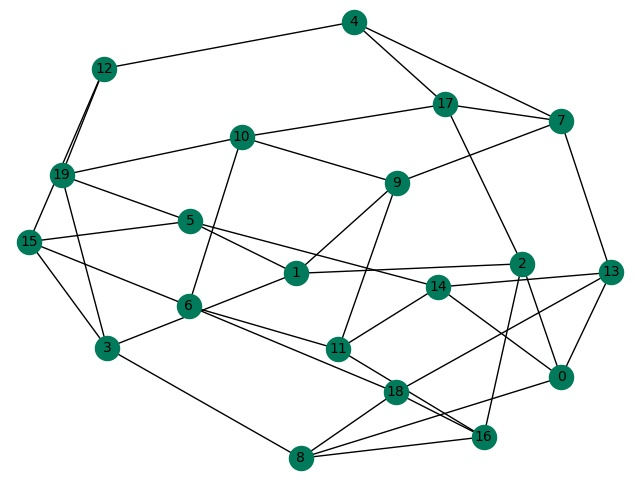
\includegraphics[width=0.9\textwidth]{4regular.jpg}
	\caption{The 4-Regular (Quartic) graph used.}
	\label{fig:4reg}
\end{figure}

\subsubsection{Deterministic Protection}

\subfile{Deterministic/DeterministicTable.tex}

\newpage

\begin{figure}[!ht]
\centering
     \begin{subfigure}[b]{0.9\textwidth}
         \centering
         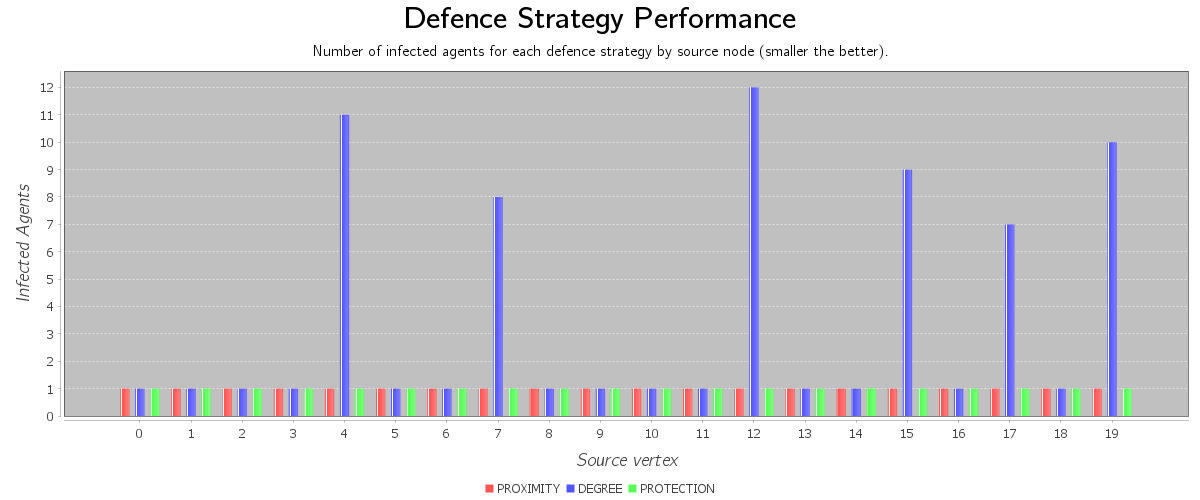
\includegraphics[width=\textwidth]{Deterministic/DeterministicInfectedChart}
         %\caption{Infected}
         \label{fig:4reg-det-infected}
     \end{subfigure}
     \vfill
     \begin{subfigure}[b]{0.9\textwidth}
         \centering
         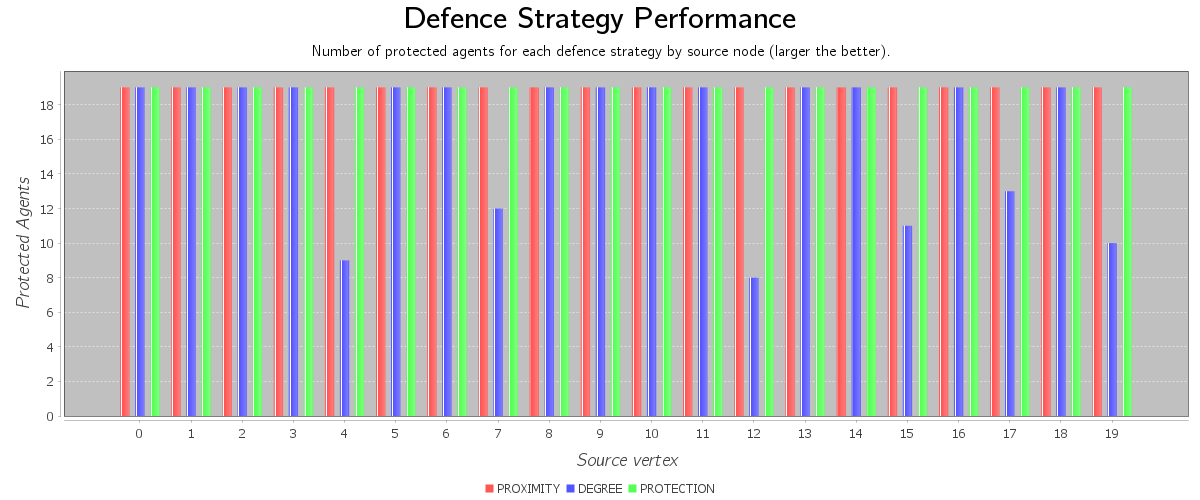
\includegraphics[width=\textwidth]{Deterministic/DeterministicProtectedChart}
         %\caption{Protected}
         \label{fig:4reg-det-protected}
     \end{subfigure}
     \vfill
     \begin{subfigure}[b]{0.9\textwidth}
         \centering
         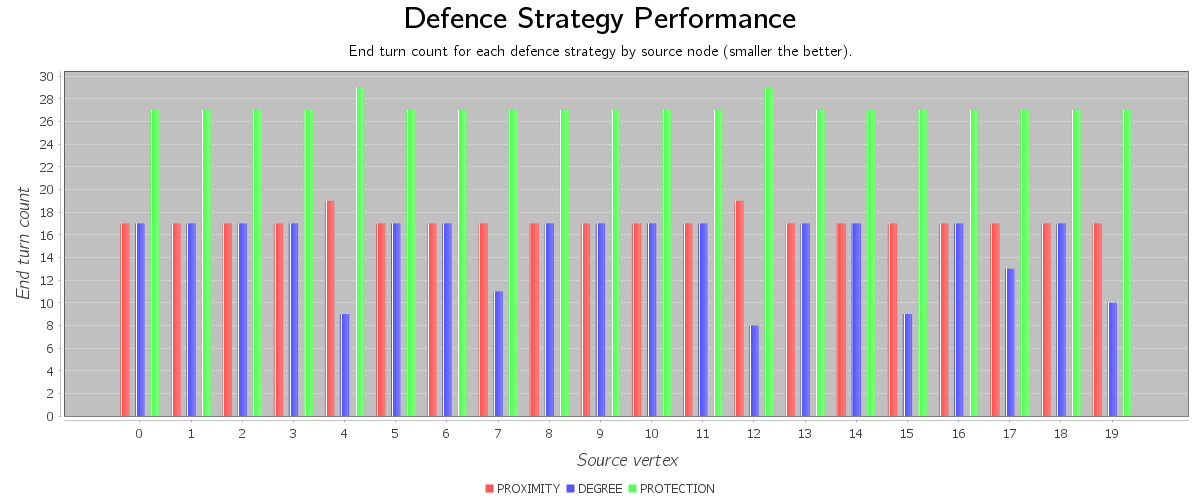
\includegraphics[width=\textwidth]{Deterministic/DeterministicEndTurnChart}
         %\caption{End Turn}
         \label{fig:4reg-det-end}
     \end{subfigure}
        \caption{Model results on a 4-Regular graph by source node for each defence strategy with deterministic initial protection allocation.}
        \label{fig:4reg-det-charts}
\end{figure}

\newpage


\subsubsection{Mixed Protection}

\subfile{Mixed/MixedTable.tex}

\newpage

\begin{figure}[!ht]
\centering
     \begin{subfigure}[b]{0.9\textwidth}
         \centering
         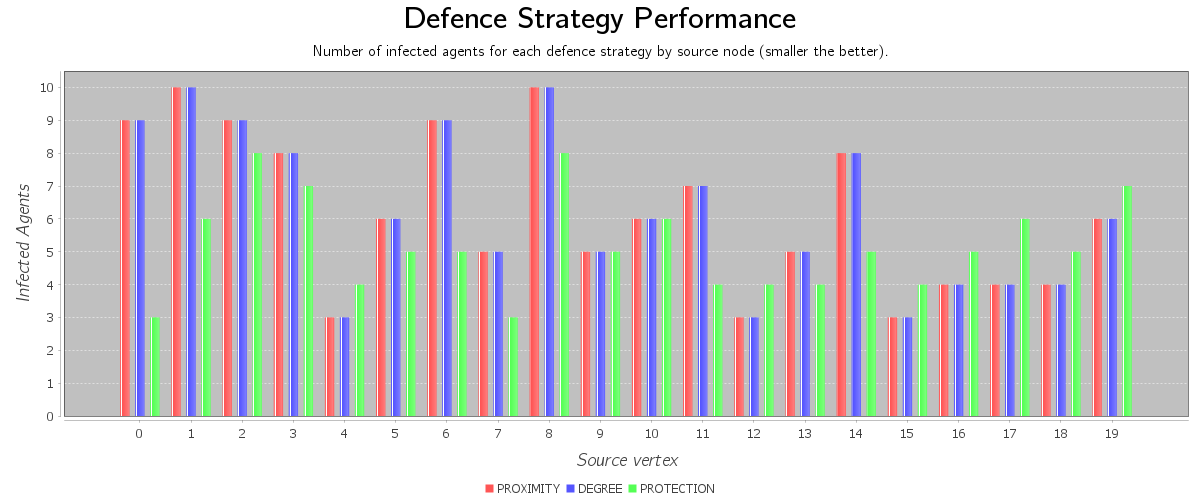
\includegraphics[width=\textwidth]{Mixed/MixedInfectedChart}
         %\caption{Infected}
         \label{fig:4reg-mix-infected}
     \end{subfigure}
     \vfill
     \begin{subfigure}[b]{0.9\textwidth}
         \centering
         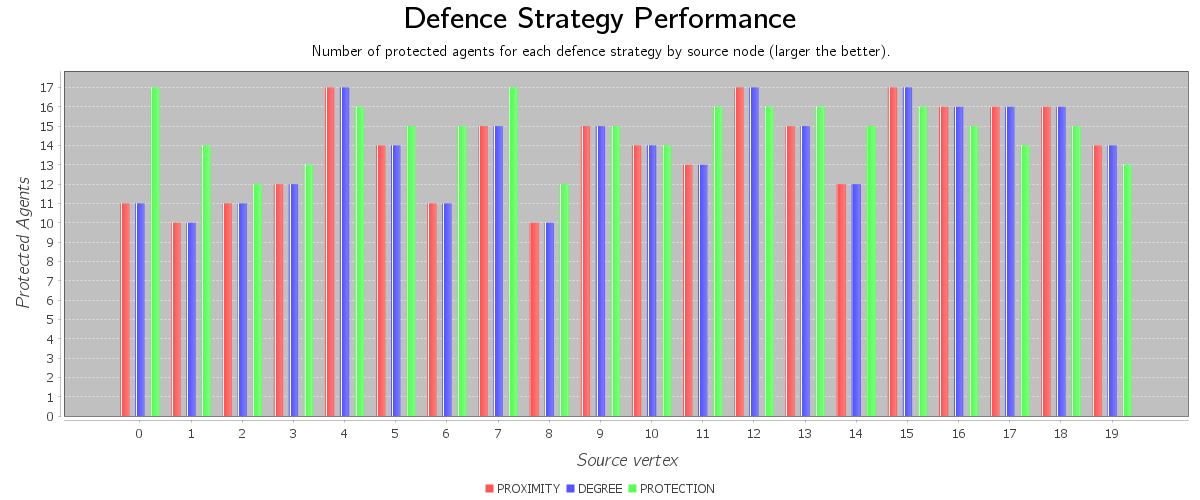
\includegraphics[width=\textwidth]{Mixed/MixedProtectedChart}
         %\caption{Protected}
         \label{fig:4reg-mix-protected}
     \end{subfigure}
     \vfill
     \begin{subfigure}[b]{0.9\textwidth}
         \centering
         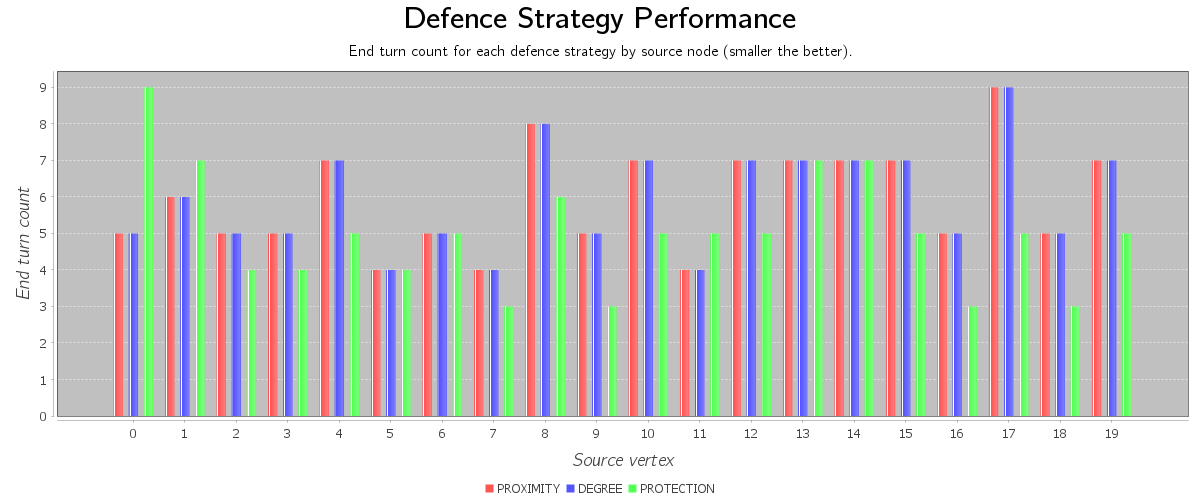
\includegraphics[width=\textwidth]{Mixed/MixedEndTurnChart}
         %\caption{End Turn}
         \label{fig:4reg-mix-end}
     \end{subfigure}
        \caption{Model results on a 4-Regular graph by source node for each defence strategy with mixed initial protection allocation.}
        \label{fig:4reg-mix-charts}
\end{figure}

\newpage 


\subsubsection{Random Protection}

\subfile{Random/RandomTable.tex}

\newpage

\begin{figure}[!ht]
\centering
     \begin{subfigure}[b]{0.9\textwidth}
         \centering
         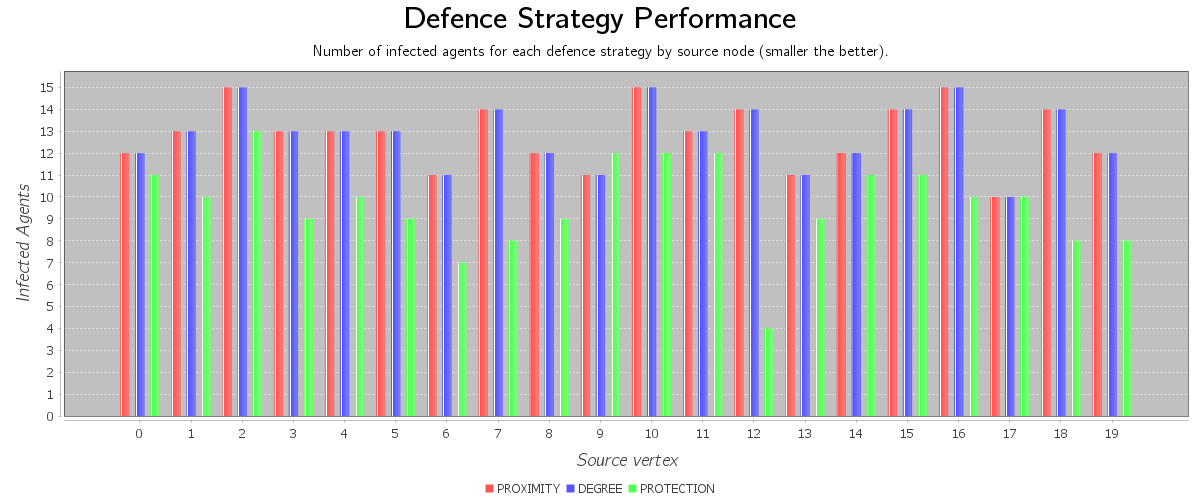
\includegraphics[width=\textwidth]{Random/RandomInfectedChart}
         %\caption{Infected}
         \label{fig:4reg-ran-infected}
     \end{subfigure}
     \vfill
     \begin{subfigure}[b]{0.9\textwidth}
         \centering
         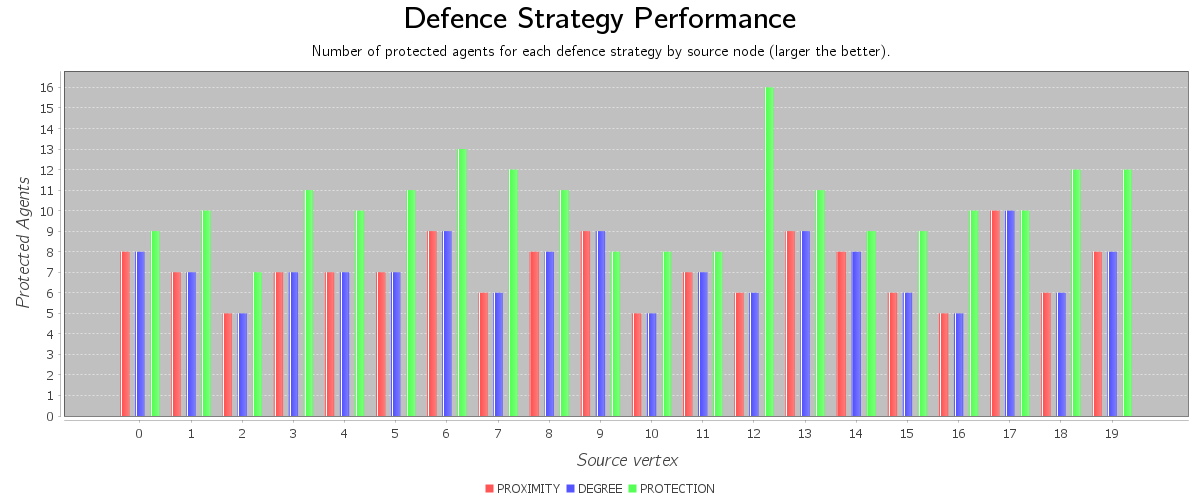
\includegraphics[width=\textwidth]{Random/RandomProtectedChart}
         %\caption{Protected}
         \label{fig:4reg-ran-protected}
     \end{subfigure}
     \vfill
     \begin{subfigure}[b]{0.9\textwidth}
         \centering
         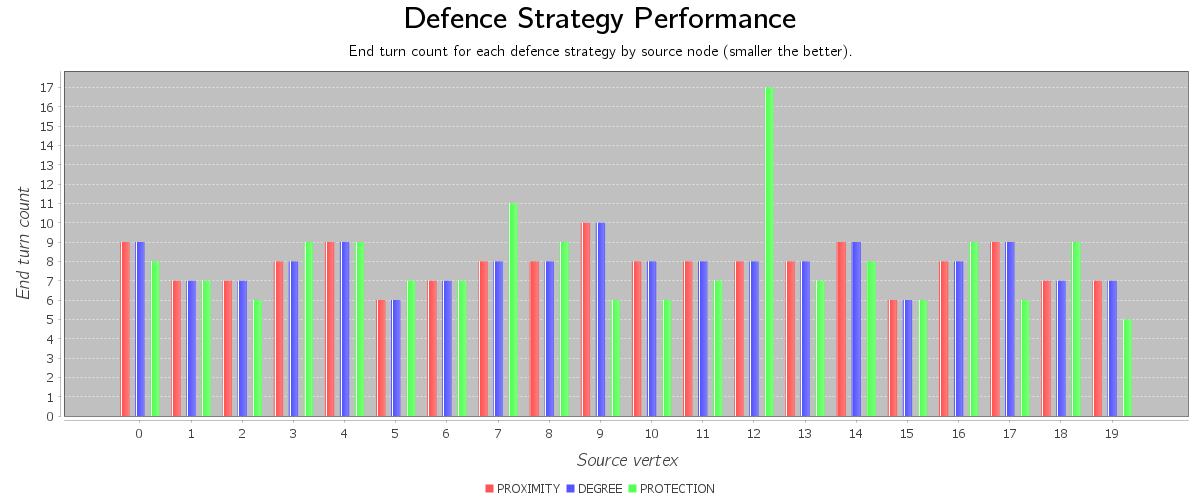
\includegraphics[width=\textwidth]{Random/RandomEndTurnChart}
         %\caption{End Turn}
         \label{fig:4reg-ran-end}
     \end{subfigure}
        \caption{Model results on a 4-Regular graph by source node for each defence strategy with random initial protection allocation.}
        \label{fig:4reg-ran-charts}
\end{figure}

\end{document}